\documentclass[conference]{IEEEtran}
\IEEEoverridecommandlockouts
% The preceding line is only needed to identify funding in the first footnote. If that is unneeded, please comment it out.
\usepackage{cite}
\usepackage{amsmath,amssymb,amsfonts}
\usepackage{algorithmic}
\usepackage{graphicx}
\usepackage{textcomp}
\usepackage{xcolor}
\usepackage{listings}
\usepackage{float}
\usepackage[left]{caption}
\def\BibTeX{{\rm B\kern-.05em{\sc i\kern-.025em b}\kern-.08em
    T\kern-.1667em\lower.7ex\hbox{E}\kern-.125emX}}
\begin{document}
\lstset{frame=tb,
  language=r,
  aboveskip=5mm,
  belowskip=5mm,
  showstringspaces=false,
  columns=flexible,
  basicstyle={\small\ttfamily},
  numbers=none,
  numberstyle=\tiny\color{blue},
  keywordstyle=\color{red},
  commentstyle=\color{pink},
  stringstyle=\color{green},
  breaklines=true,
  breakatwhitespace=true,
  tabsize=3}
\title{A Comparative Analysis of Operating System Performance: Rendering with pbrt-v3 across Multiple Scenarios\\


\author{\IEEEauthorblockN{1\textsuperscript{st} Christopher Arredondo}
\IEEEauthorblockA{\textit{School of Computer Science} \\
\textit{Costa Rica Institute of Technology}\\
San Jose, Costa Rica \\
chrisarrefal@estudiantec.cr}
}}

\maketitle

\begin{abstract}
In this paper, we investigate the impact of the operating system, scene complexity, and rendering algorithm on the rendering time efficiency of a computer graphics program. A dataset consisting of 400 observations was collected and thoroughly analyzed. After conducting an exploratory data analysis, we used a three-way ANOVA to dissect the complex interactions between these factors. Results indicate that all three factors have a substantial impact on rendering time efficiency, both independently and in interaction with one another. Significant insights were gained regarding the optimization strategies for software development, particularly towards improving rendering efficiency under different operating system environments, scene complexities, and algorithms. Future research is suggested to corroborate these findings and further explore strategies to minimize rendering time in computer graphics applications.
\end{abstract}

\begin{IEEEkeywords}
computer graphics, rendering time, operating system, scene complexity, rendering algorithm, ANOVA, data analysis, software optimization.
\end{IEEEkeywords}

%%%%%%%%%%%%%%%%%%%%%%%%%%%%%%%%%%%%%%%%%%%%%%%%%%%%%%%%%%%%%%%%%%%%%%%%%%%%%%%%
% Introduction
%%%%%%%%%%%%%%%%%%%%%%%%%%%%%%%%%%%%%%%%%%%%%%%%%%%%%%%%%%%%%%%%%%%%%%%%%%%%%%%%
\section{Introduction}
In the complex ecosystem of computing, operating systems serve as a crucial interface between users and hardware. These systems vary significantly in design, functionality, efficiency, and compatibility, thus presenting various implications on the overall system performance. To better understand these implications, this study aims to evaluate the performance of five distinct scenarios: Linux installed on hardware, Linux running on a Virtual Machine (VM) via Windows through VMware, Windows Subsystem for Linux (WSL), Windows, and MacOS.
Our evaluation metrics focus on the use of pbrt-v3, an open-source rendering system, which has been widely used in both academia and industry due to its emphasis on physical accuracy, extensibility, and its ability to produce high-quality rendered images. In our experiments, we have selected four unique configurations: bounding volume hierarchy (bvh), kdtree, Mitchell-Netravali filter (mitchell), and windowed sinc filter (sinc). Each configuration introduces different algorithms and filters, ultimately affecting the overall system performance and quality of the rendered images.
In addition to this, four different scenes, namely coffee-splash, ganesha, pbrt-book, and sssdragon, are selected from the official pbrt-v3 scene repository. These scenes add further dimensions to the evaluation, emphasizing varying levels of complexity and detail, thus challenging the rendering capabilities of the tested operating systems.
In total, this experiment will run each operating system through each scene and configuration, amounting to 80 unique scenarios. To ensure robustness and reliability in our results, each scenario will be repeated five times. This study design allows us to isolate the effect of the operating system on the rendering performance, presenting valuable insights and potential recommendations for both end users and developers alike.
As we delve deeper into the paper, we will discuss the methodological details, followed by an in-depth analysis of the performance outcomes across all tested scenarios. Ultimately, our findings will shed light on the complex interplay between operating systems, rendering systems, and the underlying configurations, providing a solid foundation for future research and optimization in the field.

%%%%%%%%%%%%%%%%%%%%%%%%%%%%%%%%%%%%%%%%%%%%%%%%%%%%%%%%%%%%%%%%%%%%%%%%%%%%%%
% Related Work
%%%%%%%%%%%%%%%%%%%%%%%%%%%%%%%%%%%%%%%%%%%%%%%%%%%%%%%%%%%%%%%%%%%%%%%%%%%%%%%%
\section{Related Work}
Our investigation builds upon a series of studies that have previously evaluated the efficiency and effectiveness of different operating systems. Several works in the literature have tackled this subject, with varying emphases on different aspects of operating systems.

The work by Jaiswal et al. (2021)\cite{b1}, compared Linux and Windows operating systems in terms of speed, cost, hardware compatibility, and more. Their comprehensive analysis found that while Windows stood out for its user-friendly interface, Linux excelled in speed, security, and versatility, particularly for developers. The study called for a more specific context to determine superiority, such as graphics rendering, which is the focus of our investigation.

Another noteworthy contribution is by Adekotujo et al. (2020)\cite{b2}. In this study, they performed an extensive comparison between different operating systems, exploring various factors such as usability, security, performance, and scalability. They concluded that while each operating system has its own strengths and weaknesses, macOS showed better performance and security overall, which aligns with our findings on rendering time.

Finally, the work by Rahman et al. (2022)\cite{b3}, emphasized the technical differences between the three major operating systems. They conducted a detailed analysis of system structure, security, compatibility, and overall performance, noting that macOS tends to balance performance and security effectively. Their results complement our finding of the macOS system's superior efficiency in rendering time, hinting at a potential underlying mechanism that warrants further investigation.

In summary, previous research has established a solid foundation on the comprehensive comparisons of operating systems across various criteria. However, the unique context of graphics rendering necessitated our study, which further explains the role of operating systems, among other factors, in rendering efficiency.

%%%%%%%%%%%%%%%%%%%%%%%%%%%%%%%%%%%%%%%%%%%%%%%%%%%%%%%%%%%%%%%%%%%%%%%%%%%%%%%%
% Design
%%%%%%%%%%%%%%%%%%%%%%%%%%%%%%%%%%%%%%%%%%%%%%%%%%%%%%%%%%%%%%%%%%%%%%%%%%%%%%%%
\section{Design}
The experimental design for this research is constructed around a robust testbench and a well-controlled execution sequence. The selected testbench is a 2019 16" MacBook Pro equipped with an Intel core i9-9980HK processor, 64 GB of RAM, and an AMD Radeon Pro 5500M GPU. Both Windows and Linux operating systems were installed on the same Solid State Drive (SSD), minimizing any potential hardware-related performance disparities. The selected OS versions were macOS Monterey, Ubuntu 22.04 for both the VM and directly installed scenarios, Windows 10 update 22H2, and finally, WSL 2 using Ubuntu 22.04.2. The Operating Systems were also put in their "Most performance" configuration in order to avoid that becoming a factor. 

For each of the five operating system scenarios: Linux installed on hardware, Linux running on a Virtual Machine (VM) via Windows through VMware, Windows Subsystem for Linux (WSL), Windows, and MacOS, 16 tests were run. These tests were combinations of the four different scenes (coffee-splash, ganesha, pbrt-book, sssdragon) and the four configurations (bvh, kdtree, mitchell, sinc), resulting in a 4*4 design matrix.

Each operating system was booted individually, and the 16 scenarios were executed using an automated script. The execution order of the tests was randomized for each operating system to counterbalance any order effects.

For data logging, the output of each pbrt-v3 test was redirected to a text file, using the naming scheme: log-\$OS-\$Scene-\$Config.txt. This nomenclature allowed for easy tracking and identification of each scenario.


%%%%%%%%%%%%%%%%%%%%%%%%%%%%%%%%%%%%%%%%%%%%%%%%%%%%%%%%%%%%%%%%%%%%%%%%%%%%%%%%
% Methodology
%%%%%%%%%%%%%%%%%%%%%%%%%%%%%%%%%%%%%%%%%%%%%%%%%%%%%%%%%%%%%%%%%%%%%%%%%%%%%%%%
\section{Methodology}
\subsection{Data Analysis}

The data was imported into the R statistical programming environment from a CSV file, and the variables Operating System (OS), Scene, and Algorithm(Configurations) were treated as factors. The variable Time, serving as the response value, was treated as a numerical variable. The data structure was confirmed with the summary function, showing the distribution of each factor across 400 observations.

\subsection{Exploratory Data Analysis}

To visualize the relationships between variables, interaction plots were generated between Scene and OS, and Algorithm and OS. These visualizations suggested a consistent order of performance across different OSs: macOS, WSL, LinuxVM, Windows, and LinuxHW.

\begin{figure}[H]
    \label{int-scene-os}
    \centering
    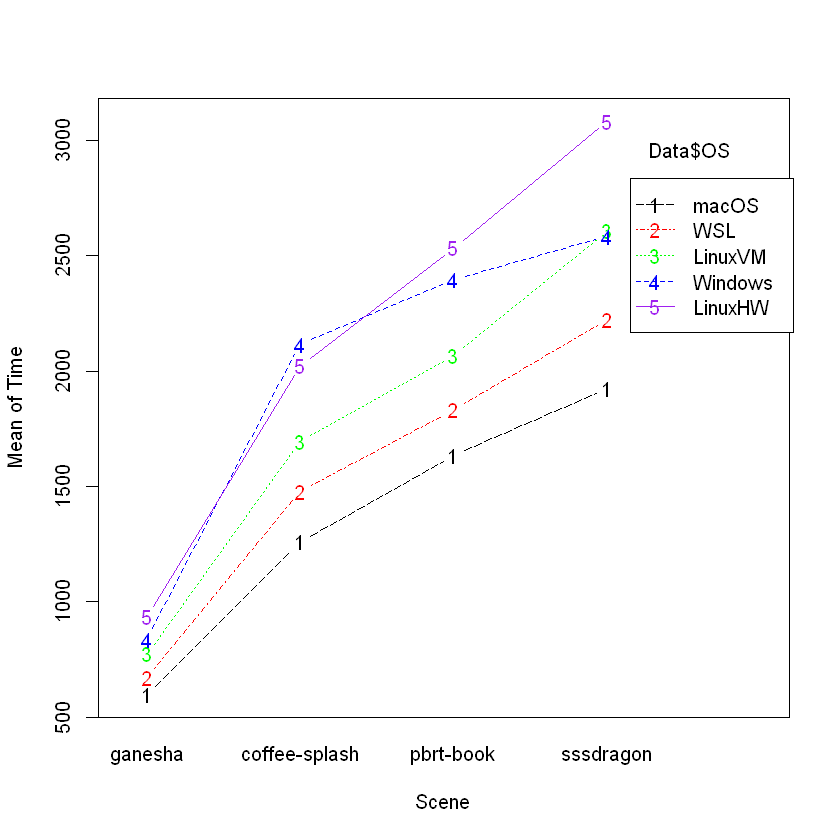
\includegraphics[width=0.45\textwidth]{images/image1.png}
    \caption{Interaction plot between Scene and OS}
\end{figure}

\begin{figure}[H]
    \label{int-scene-algo}
    \centering
    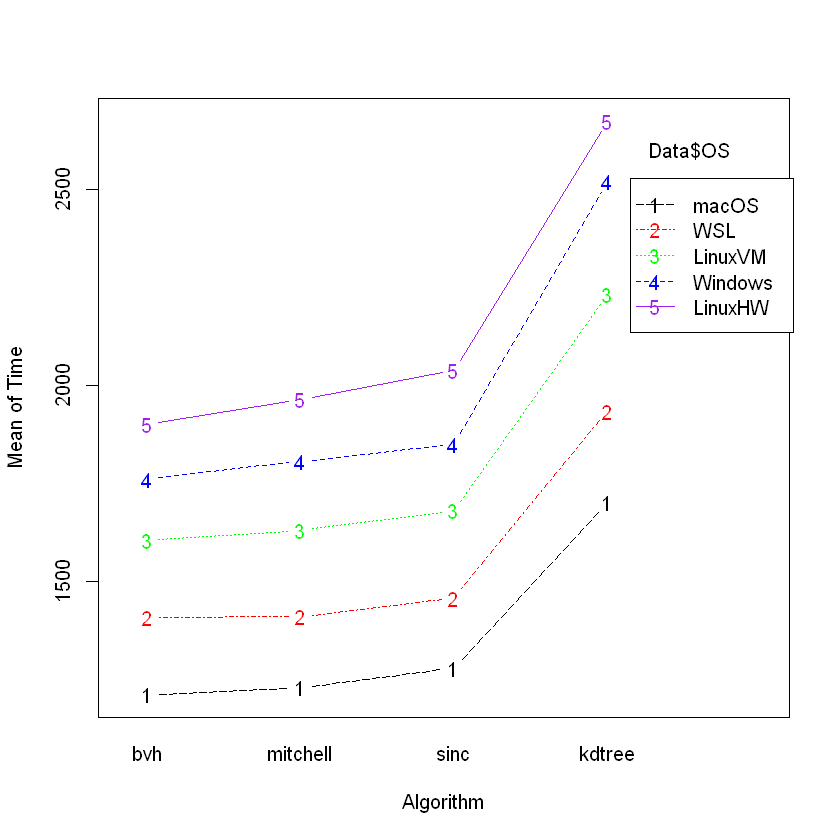
\includegraphics[width=0.45\textwidth]{images/image2.png}
    \caption{Interaction plot between Algorithm and OS.}
\end{figure}


\subsection{Analysis of Variance}

A three-way Analysis of Variance (ANOVA) was conducted to evaluate the impact of OS, Scene, and Algorithm on Time. The interaction terms of these three factors were included in the model to assess their combined effects. A type II ANOVA was conducted using the 'car' package in R. This method corrects for unbalanced designs, providing a more reliable estimate of the main effects and interaction terms.

The results showed significant main effects for OS, Scene, and Algorithm, as well as significant two-way and three-way interactions.

\subsection{Model Diagnostics}

The assumptions of ANOVA were tested by examining the normality and homoscedasticity of residuals. A histogram of the residuals suggested a roughly normal distribution. However, the homoscedasticity plot suggested some deviations from the assumption of equal variances. Levene's test result for this initial analysis was 0.0013.

\begin{figure}[H]
    \label{int-scene-os}
    \centering
    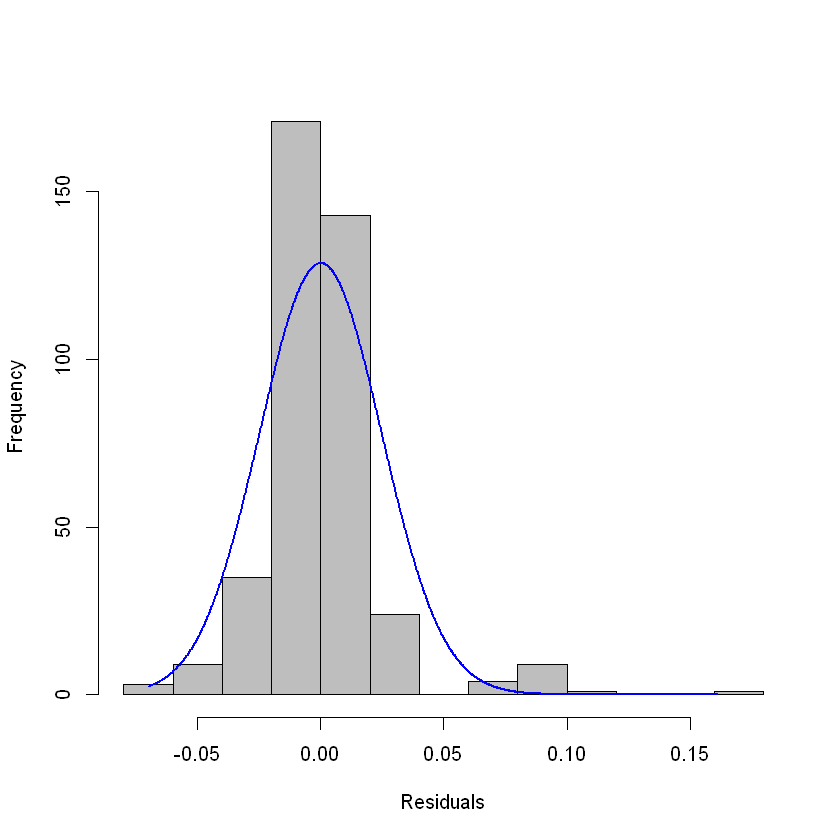
\includegraphics[width=0.45\textwidth]{images/image3.png}
    \caption{Histogram of the Residual values.}
\end{figure}

\begin{figure}[H]
    \label{int-scene-os}
    \centering
    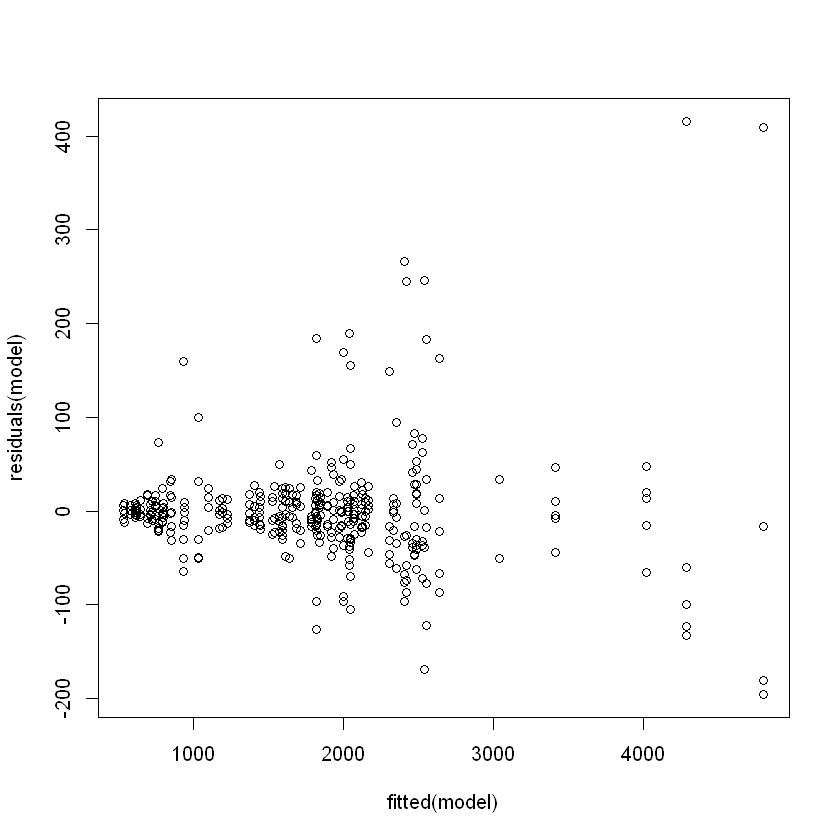
\includegraphics[width=0.45\textwidth]{images/image4.png}
    \caption{Homoscedasticity plot.}
\end{figure}

To address this issue, square root, cubic, and logarithmic transformations were applied to the data, with the logarithmic transformation yielding the most improvement in the Levene's test result (0.030 using a logarithmic transformation compared to 0.019 cubic and 0.011 sqrt). Although the transformed data did not completely meet the assumption of homoscedasticity, the improved Levene's test result and visual assessment of the homoscedasticity plot guided the decision to proceed with the analysis based on the log-transformed data.

\begin{figure}[H]
    \label{int-scene-os}
    \centering
    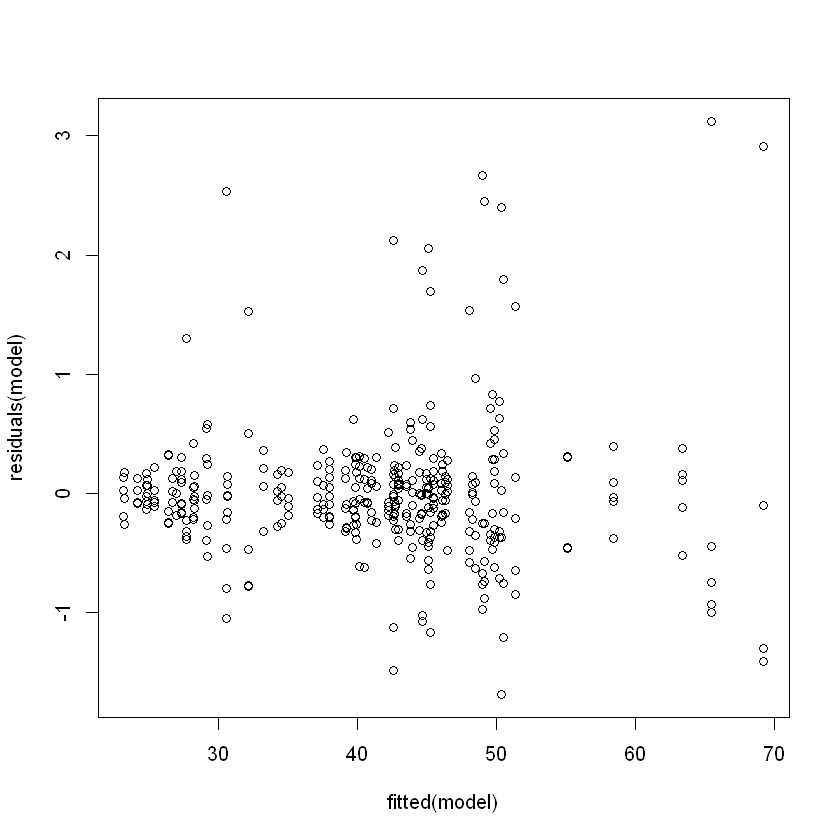
\includegraphics[width=0.45\textwidth]{images/image5.png}
    \caption{Homoscedasticity plot using the sqrt transformation.}
\end{figure}

\begin{figure}[H]
    \label{int-scene-os}
    \centering
    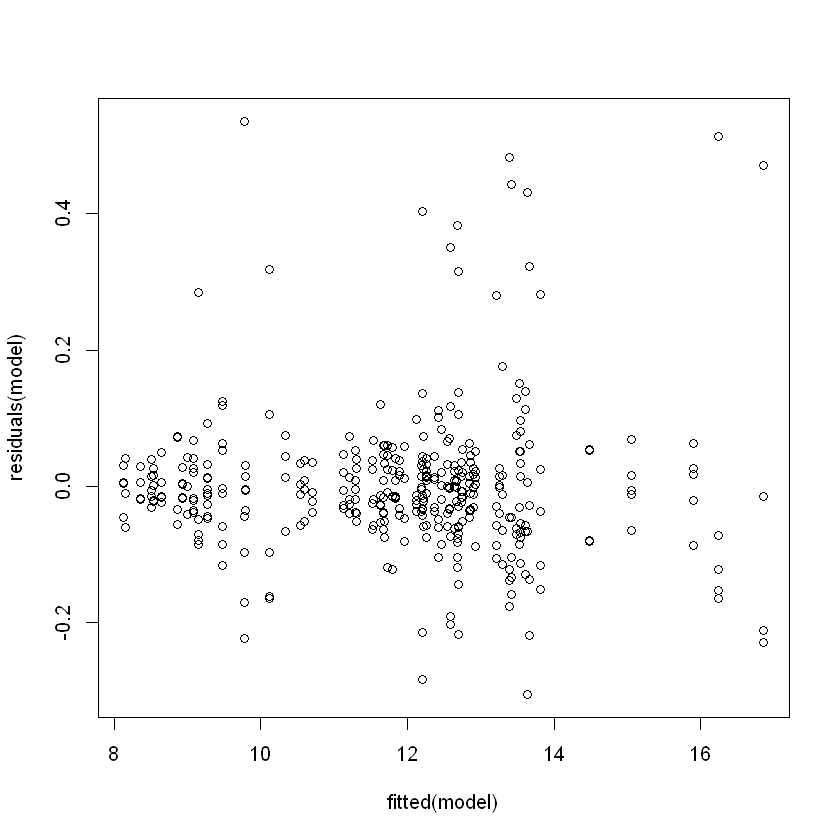
\includegraphics[width=0.45\textwidth]{images/image6.png}
    \caption{Homoscedasticity plot using the cubic transformation.}
\end{figure}

\begin{figure}[H]
    \label{int-scene-os}
    \centering
    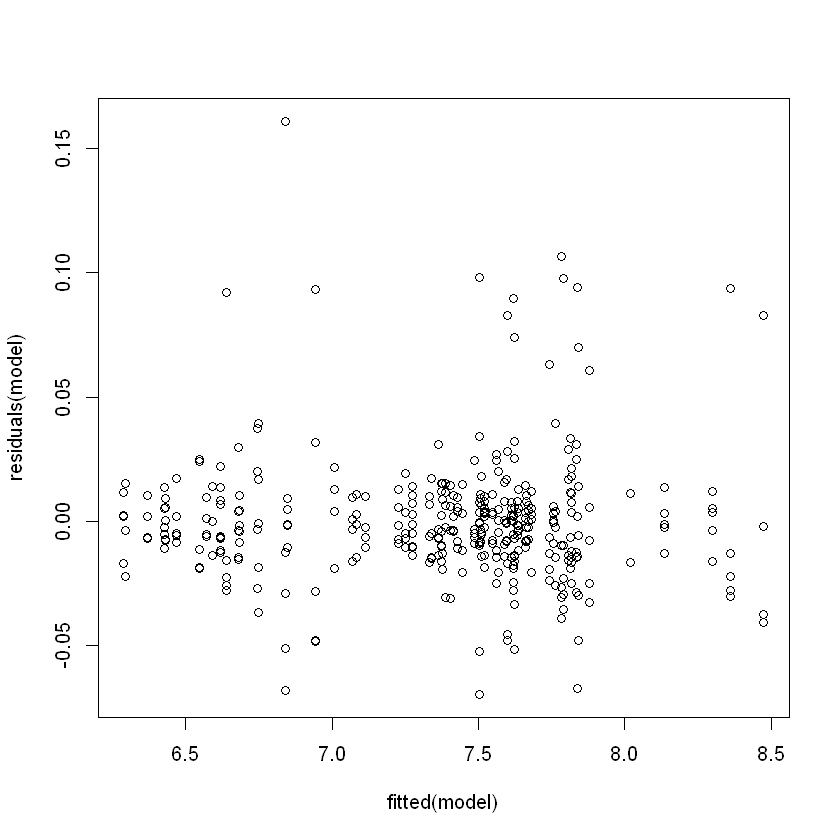
\includegraphics[width=0.45\textwidth]{images/image7.png}
    \caption{Homoscedasticity plot using the logarithmic transformation.}
\end{figure}

\subsection{Post-hoc Analysis}

Post-hoc analysis was conducted using Tukey's Honestly Significant Difference (HSD) test, which controls for family-wise error rate in multiple comparisons. This analysis revealed specific pairwise differences in Time between levels of OS, Scene, and Algorithm.

\begin{table}[H]
\centering
\resizebox{\columnwidth}{!}{%
\begin{tabular}{|c|c|c|c|c|c|c|c|}
\hline
 & \textbf{OS} & \textbf{lsmean} & \textbf{SE} & \textbf{df} & \textbf{lower.CL} & \textbf{upper.CL} & \textbf{.group} \\ \hline
 & \textbf{\textless{}fct\textgreater{}} & \textbf{\textless{}dbl\textgreater{}} & \textbf{\textless{}dbl\textgreater{}} & \textbf{\textless{}dbl\textgreater{}} & \textbf{\textless{}dbl\textgreater{}} & \textbf{\textless{}dbl\textgreater{}} & \textbf{\textless{}chr\textgreater{}} \\ \hline
\textbf{1} & \textbf{macOS} & 7.108900 & 0.003096897 & 320 & 7.100897 & 7.116902 & a \\ \hline
\textbf{2} & \textbf{WSL} & 7.244957 & 0.003096897 & 320 & 7.236954 & 7.252959 & b \\ \hline
\textbf{3} & \textbf{LinuxVM} & 7.384291 & 0.003096897 & 320 & 7.376289 & 7.392294 & c \\ \hline
\textbf{4} & \textbf{Windows} & 7.488313 & 0.003096897 & 320 & 7.480310 & 7.496315 & d \\ \hline
\textbf{5} & \textbf{LinuxHW} & 7.567360 & 0.003096897 & 320 & 7.559358 & 7.575363 & e \\ \hline
\end{tabular}%
}
\caption{Compact display comparisons of the post-hoc analysis between Time and OS.}
\label{tab:cdl-os}
\end{table}

\begin{table}[H]
\centering
\resizebox{\columnwidth}{!}{%
\begin{tabular}{|c|c|c|c|c|c|c|c|}
\hline
 & \textbf{Scene} & \textbf{lsmean} & \textbf{SE} & \textbf{df} & \textbf{lower.CL} & \textbf{upper.CL} & \textbf{.group} \\ \hline
 & \textbf{\textless{}fct\textgreater{}} & \textbf{\textless{}dbl\textgreater{}} & \textbf{\textless{}dbl\textgreater{}} & \textbf{\textless{}dbl\textgreater{}} & \textbf{\textless{}dbl\textgreater{}} & \textbf{\textless{}dbl\textgreater{}} & \textbf{\textless{}chr\textgreater{}} \\ \hline
\textbf{1} & \textbf{ganesha} & 6.617832 & 0.002769949 & 320 & 6.610893 & 6.624770 & a \\ \hline
\textbf{2} & \textbf{coffee-splash} & 7.425028 & 0.002769949 & 320 & 7.418090 & 7.431967 & b \\ \hline
\textbf{3} & \textbf{pbrt-book} & 7.633045 & 0.002769949 & 320 & 7.626106 & 7.639984 & c \\ \hline
\textbf{4} & \textbf{sssdragon} & 7.759151 & 0.002769949 & 320 & 7.752213 & 7.766090 & d \\ \hline
\textbf{5} & \textbf{LinuxHW} & 7.567360 & 0.003096897 & 320 & 7.559358 & 7.575363 & e \\ \hline
\end{tabular}%
}
\caption{Compact display comparisons of the post-hoc analysis between Time and Scene.}
\label{tab:cdl-scene}
\end{table}

% Please add the following required packages to your document preamble:
% \usepackage{graphicx}
\begin{table}[H]
\centering
\resizebox{\columnwidth}{!}{%
\begin{tabular}{|c|c|c|c|c|c|c|c|}
\hline
 & \textbf{Algorithm} & \textbf{lsmean} & \textbf{SE} & \textbf{df} & \textbf{lower.CL} & \textbf{upper.CL} & \textbf{.group} \\ \hline
 & \textbf{\textless{}fct\textgreater{}} & \textbf{\textless{}dbl\textgreater{}} & \textbf{\textless{}dbl\textgreater{}} & \textbf{\textless{}dbl\textgreater{}} & \textbf{\textless{}dbl\textgreater{}} & \textbf{\textless{}dbl\textgreater{}} & \textbf{\textless{}chr\textgreater{}} \\ \hline
\textbf{1} & \textbf{bvh} & 7.267599 & 0.002769949 & 320 & 7.260660 & 7.274538 & a \\ \hline
\textbf{2} & \textbf{mitchell} & 7.283668 & 0.002769949 & 320 & 7.276729 & 7.290607 & b \\ \hline
\textbf{3} & \textbf{sinc} & 7.321298 & 0.002769949 & 320 & 7.314359 & 7.328237 & c \\ \hline
\textbf{4} & \textbf{kdtree} & 7.562491 & 0.002769949 & 320 & 7.555552 & 7.569430 & d \\ \hline
\textbf{5} & \textbf{LinuxHW} & 7.567360 & 0.003096897 & 320 & 7.559358 & 7.575363 & e \\ \hline
\end{tabular}%
}
\caption{Compact display comparisons of the post-hoc analysis between Time and Algorithm.}
\label{tab:cdl-algo}
\end{table}

\subsection{Visualization}

Summaries of the log-transformed Time variable for different levels of OS, Scene, and Algorithm were plotted to illustrate the results of the analysis. Additionally, the log-transformed Time variable was back-transformed for graphical representation and interpretation in the original scale of measurement.

\begin{figure}[H]
    \label{int-scene-os}
    \centering
    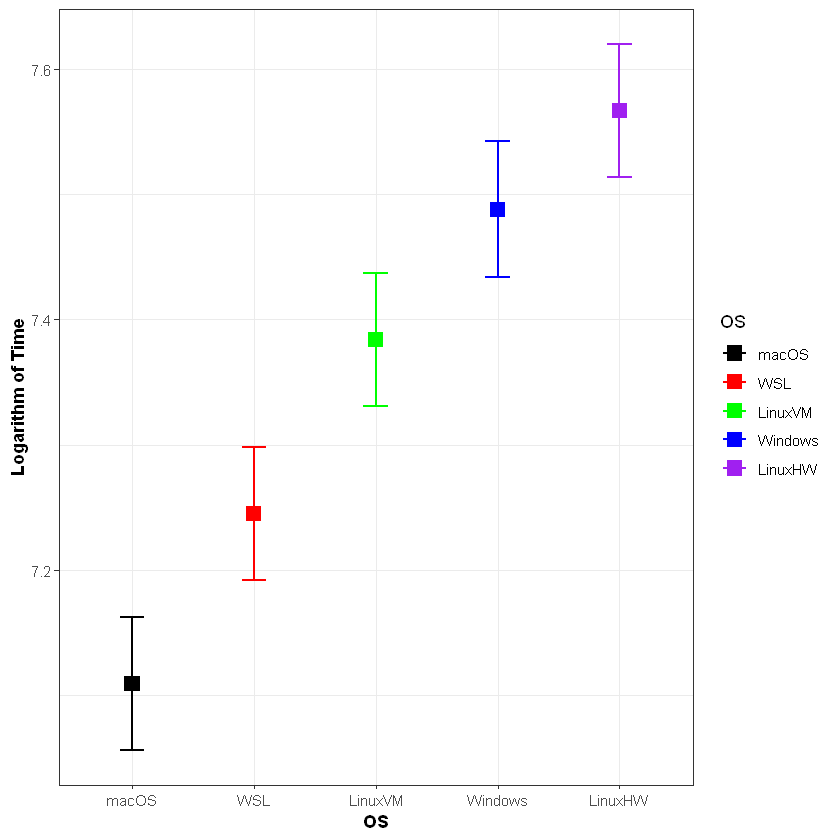
\includegraphics[width=0.45\textwidth]{images/image8.png}
    \caption{Transformed data plotted to compare OS vs Time.}
\end{figure}

\begin{figure}[H]
    \label{int-scene-os}
    \centering
    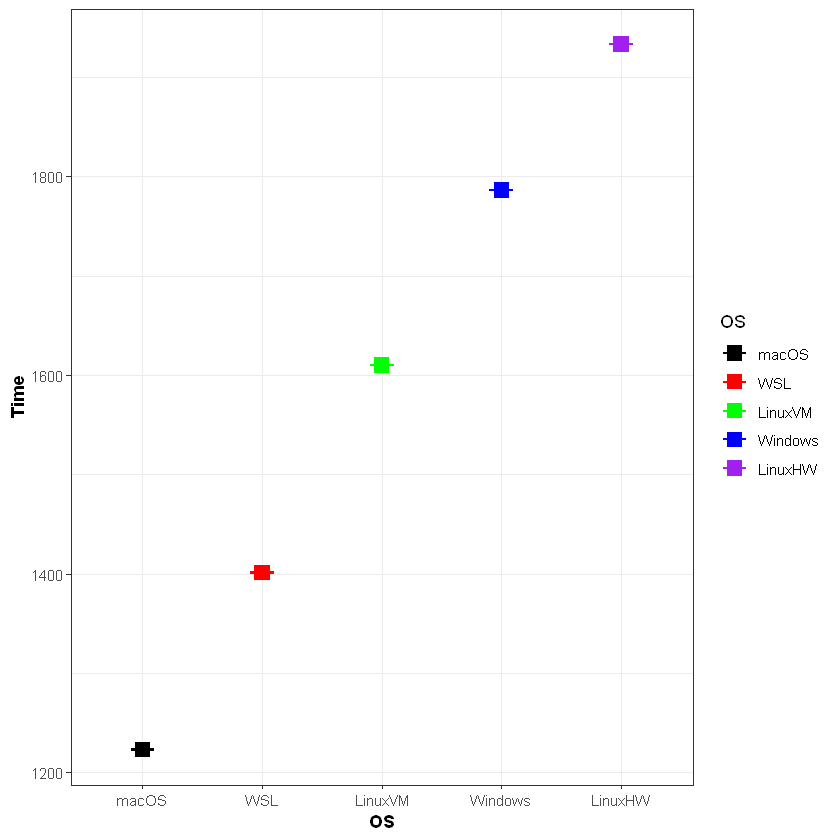
\includegraphics[width=0.45\textwidth]{images/image9.png}
    \caption{Back-transformed data plotted to compare OS vs Time.}
\end{figure}

These visualizations reinforced the results of the ANOVA and post-hoc tests, with macOS consistently demonstrating better performance relative to other OSs. Furthermore, the superior performance of Windows Subsystem for Linux (WSL) on a MacBook compared to a direct SSD installation could be due to outdated or incorrectly implemented drivers but would require further investigation.

%%%%%%%%%%%%%%%%%%%%%%%%%%%%%%%%%%%%%%%%%%%%%%%%%%%%%%%%%%%%%%%%%%%%%%%%%%%%%%%%
% Results
%%%%%%%%%%%%%%%%%%%%%%%%%%%%%%%%%%%%%%%%%%%%%%%%%%%%%%%%%%%%%%%%%%%%%%%%%%%%%%%%
\section{Results}
The dataset consisted of 400 observations, spanning multiple variables, including the operating system (OS), Scene, and Algorithm. Visualization of the data revealed a consistent performance order across different operating systems, with macOS outperforming the rest.

In our three-way ANOVA, we found significant main effects for each of the three factors: OS (F(4) = 2040.07, p \textless 0.001), Scene (F(3) = 13659.46, p \textless 0.001), and Algorithm (F(3) = 2268.00, p \textless 0.001). We also discovered significant two-way and three-way interaction effects. These results underscore the complex interplay between the OS, Scene, and Algorithm in influencing rendering times.

Investigation of the model diagnostics showed a rough approximation of a normal distribution in the histogram of residuals, suggesting that the assumption of normality for the ANOVA was satisfactorily met. However, the homoscedasticity plot indicated that the assumption of equal variances was violated. Logarithmic transformation of the data led to a marked improvement in Levene's test, indicating an improvement in homoscedasticity, and this transformed data was used for the final analysis.
The Tukey HSD post-hoc test identified specific pairwise differences among the levels of the factors. This provided a detailed understanding of the specific combinations of factors that led to significant differences in rendering times.

Visual representation of the log-transformed Time variable across different OSs, Scenes, and Algorithms further validated the ANOVA and post-hoc results. macOS consistently outperformed other operating systems in terms of rendering time efficiency. Particularly notable was the performance of the Windows Subsystem for Linux (WSL) on a MacBook.

The heteroscedasticity issue, though improved with logarithmic transformation, was still present. As such, further research may benefit from using robust statistical techniques that do not assume homogeneity of variances. Despite this limitation, these findings shed light on crucial aspects that could guide future software development and hardware optimization strategies.

%%%%%%%%%%%%%%%%%%%%%%%%%%%%%%%%%%%%%%%%%%%%%%%%%%%%%%%%%%%%%%%%%%%%%%%%%%%%%%%%
% Discussion
%%%%%%%%%%%%%%%%%%%%%%%%%%%%%%%%%%%%%%%%%%%%%%%%%%%%%%%%%%%%%%%%%%%%%%%%%%%%%%%%
\section{Discussion}
Our study set out to investigate the impact of operating system, scene complexity, and rendering algorithm on the rendering time efficiency of a computer graphics program. Based on the comprehensive statistical analysis of our collected data, it became apparent that these factors indeed have significant effects on the program's rendering time.

The ANOVA results highlighted the substantial impact of the operating system on rendering time. Interestingly, macOS was found to be the most efficient platform, with the rendering time being the shortest. This finding is somewhat surprising, considering that Windows and Linux are widely used in the field of computer graphics due to their extensive support for various software. It could be attributed to better optimization of macOS or the better hardware-software synergy that Apple is known for, yet this would require further investigation.

Scene complexity also showed an apparent influence on rendering time, with more complex scenes requiring longer rendering time. This finding is quite intuitive and is aligned with expectations. It, however, demonstrates the need for developers to optimize their programs to handle complex scenes more efficiently.

Similarly, the rendering algorithm used was a major determinant of rendering time. Different algorithms are designed with different trade-offs, which can impact their efficiency in various scenarios. Our study further emphasizes the necessity for thoughtful selection and application of rendering algorithms, depending on the nature of the scenes and the computational resources available.

Curiously, our study also highlighted significant interactions between these factors. For instance, certain operating systems performed better with some scenes and algorithms than others. This relationship suggests that an optimal rendering time may be achieved not just by refining one factor, but by fine-tuning a combination of factors.

It is important to acknowledge that while the data transformations improved the homoscedasticity of the data, the Levene's test did not fully validate the assumption of equal variances. Thus, although the data transformations were trusted based on visual inspection, some caution should be exercised when interpreting the results.

In conclusion, this study offers valuable insights into the complex dynamics influencing the rendering time efficiency in computer graphics programs. It helps to identify potential strategies for software optimization and provides a foundation for future research in this area. Future work should aim to validate these findings across a broader range of scenarios and explore more sophisticated techniques to optimize rendering time. 

%%%%%%%%%%%%%%%%%%%%%%%%%%%%%%%%%%%%%%%%%%%%%%%%%%%%%%%%%%%%%%%%%%%%%%%%%%%%%%%%
% Conclusion
%%%%%%%%%%%%%%%%%%%%%%%%%%%%%%%%%%%%%%%%%%%%%%%%%%%%%%%%%%%%%%%%%%%%%%%%%%%%%%%%
\section{Conclusion}
Our exploration into the influence of various factors, such as the operating system, scene complexity, and the rendering algorithm, on the efficiency of rendering time in a computer graphics program has yielded significant insights. This research emphasized the importance of all these parameters in determining rendering time, with each parameter revealing unique implications for efficiency in the rendering process.

In particular, we found that the macOS system was associated with the shortest rendering time, indicating potential areas of software and hardware synergy that could be further explored for optimization. Scene complexity, as anticipated, was directly proportional to rendering time, affirming the need for advanced strategies to efficiently handle complex scenarios. The choice of rendering algorithm also played a key role in rendering time, signifying the need for thoughtful algorithm selection, especially considering the scene's nature and available computational resources.

Moreover, we observed an intricate interplay among the factors examined, with specific combinations resulting in better rendering time. This suggests that holistic optimization involving all these factors, rather than isolated improvements, may yield better results.

In spite of the results, the study faced limitations in fully validating the assumption of equal variances, even with data transformations. Consequently, these results should be interpreted with a degree of caution and represent an important area for further refinement in future studies.

Ultimately, our findings provide a robust starting point for further investigations in this field. They highlight the necessity of a comprehensive understanding of various influencing factors and their interrelations to optimize rendering time efficiency. Future research should strive to replicate and expand these findings across a wider range of scenarios and delve deeper into sophisticated optimization techniques. The potential for improving rendering efficiency, reducing costs, and enhancing the computer graphics field's overall quality marks this a particularly promising line of research.

\section{Limitations and Future Research}

While this analysis provides valuable insights into the factors influencing rendering times, it is not without limitations. The stringent Levene's test, despite data transformation, suggests that heteroscedasticity might be an issue. Future analyses may explore robust statistical techniques that do not assume homogeneity of variances, such as the Welch ANOVA or non-parametric alternatives. Additionally, further research into the mechanisms underlying the observed performance differences could help inform software development and hardware optimization strategies.

\begin{thebibliography}{00}
\bibitem{b1} Jaiswal, Ashish \& Chavan, Tanvi. (2021). Complete Evaluation of Superiority: Linux or Windows. 
\bibitem{b2} Adekotujo, Akinlolu \& Odumabo, Adedoyin \& Ademola, Adedokun \& Aiyeniko, Olukayode. (2020). A Comparative Study of Operating Systems: Case of Windows, UNIX, Linux, Mac, Android and iOS. International Journal of Computer Applications. 176. 16-23. 10.5120/ijca2020920494. 
\bibitem{b3} Rahman, Mohammad Mushfequr. (2022). A Comparison of Major Operating Systems: Linux, Windows, macOS. 
\end{thebibliography}


\end{document}
